\documentclass[paper=a4,11pt,titlepage,twoside=true,headings=normal,numbers=noenddot,captions=tableabove,listof=totoc,index=totoc,bibliography=totoc]{scrreprt}
%\usepackage{amsmath} % abgesetzte Formeln zentriert in der Zeile
%\usepackage[fleqn,intlimits]{amsmath} % [fleqn] abgesetzte Formeln mit festem Abstand zum linken Rand
\usepackage[reqno,intlimits]{amsmath} % [reqno] um die gleichungsnummerierung rechts zu haben
% intlimits: Grenzen für Integrale unterhalb und oberhalb des Zeichens
\usepackage{amssymb}
\usepackage{array}
\usepackage[ngerman]{babel}
\usepackage[ngerman]{varioref}
\usepackage[T1]{fontenc} 
\usepackage[utf8]{inputenc}
%---------------------------
\usepackage{booktabs}
\usepackage{calc}
\usepackage{cancel}
\usepackage[labelfont={footnotesize,sf,bf},textfont={footnotesize,sf}]{caption} %Format (Textgröße, Textform) für Bildtext 
%normalsize
%scriptsize
% sc --> smallcaps
% bf --> bold face
% sf --> sans serif
%\usepackage{cleveref} % löscht labels!!!!!!!!!!
%\usepackage{cite} %inkompatibel mit biblatex
\usepackage[table]{xcolor}
%\usepackage{colortbl}
\usepackage[right]{eurosym}
%\usepackage{caption2} %nicht zusammen mit sidecap
%\usepackage{exscale}
\usepackage{ellipsis}
\usepackage{graphicx}
\usepackage{float}
%\usepackage{floatflt}
%----------------------------------------
\usepackage{gensymb} %-----------
%\usepackage{helvet}
\usepackage{csquotes}
\usepackage{listings}
\usepackage{longtable}
\usepackage{lastpage}  %----------
\usepackage{lscape}
\usepackage{lmodern}  %-- Silbentrennung
%\usepackage{mathpazo} % andere mathematische Symbol
\usepackage{makeidx}
%\usepackage{minitoc}
\usepackage{multirow}
\usepackage{multicol}
%\usepackage[intoc]{nomencl}   % zwei Spalten beim Formelzeichenverzeichnis
\usepackage[german,intoc]{nomentbl} %vier Spalten bei Formelzeichenverzeichnis
\usepackage{nicefrac} %----
%\usepackage{picins} %----------
\usepackage{paralist} %--------
\usepackage{parallel}  %----------
\usepackage{pdfpages} %-------
% Define user colors using the RGB model
%\usepackage{colortbl}
%\definecolor{dunkelgrau}{rgb}{0.8,0.8,0.8}
%\definecolor{hellgrau}{rgb}{0.95,0.95,0.95}
%\usepackage{pgfplots}
\usepackage[figuresright]{rotating} 
\usepackage{scrlayer-scrpage}
%\usepackage[innercaption]{sidecap} %Beschriftung neben Bild, Tabelle, Mittelbach S333 %----------
%\usepackage{sistyle}
%\usepackage[locale=DE]{siunitx} %nicht zusammen mit sistyle %---------
\usepackage[locale=DE,per-mode=symbol,parse-numbers=false]{siunitx} %nicht zusammen mit sistyle %---------
\usepackage[font={scriptsize,sl},captionskip=3pt]{subfig} % für die Unterbilder %---------
\usepackage{shortvrb}
\usepackage{tablefootnote}
\usepackage{tabularx}
\usepackage{tabulary}
\usepackage{textcomp}
\usepackage{tocbasic}
%\usepackage{tikz}
\usepackage{times} 
\usepackage{units} %----------
\usepackage{url}
\usepackage{wrapfig} %----------
\usepackage{xr-hyper}
\usepackage{arydshln} %für \hdashline[5pt/2pt] % muss am Ende stehen, sonst gibt es Probleme mit xcolor
\usepackage{hyperref} % muss am Schluss stehen
\hypersetup{linkcolor={0 1 1}, linkbordercolor={1 1 1}, citebordercolor={1 1 1}} % setzt Linkboxen auf Farbe "`weiß"'
%\usepackage{bm}
%\usepackage[toc,symbols]{glossaries} %---------- muss nach hyperref stehen
\usepackage[nonumberlist, acronym, toc, section]{glossaries} % muss nach hypersetup stehen
%----------------
%\usepackage{romannum} % Seitenzahlen in römischen Ziffern
%\usepackage{adjustbox}
\usepackage{scrhack}
\usepackage[style=numeric, citestyle=numeric, backend=biber]{biblatex}
%-------------------------
 %\renewcommand{\captionlabelfont}{\sffamily} %für "Abbildung" und "Tabelle"
 %\renewcommand{\captionfont}{\sffamily\small} %für den Text der Bildunterschriften
%  \renewcommand{\captionlabelfont}{\sffamily} 
%  \renewcommand{\captionfont}{\sffamily} %\renewcommand{\normalfont}{\sffamily} %für die Überschriften
% Fettdruck der Bezeichnung Abbildung, Tabelle
%\renewcommand{\captionlabelfont}{\bfseries}
%---------------------------------------------
%------------------ Schrifttyp in der Kopf- und Fusszeilen
\setkomafont{pageheadfoot}{\footnotesize\sffamily}
%---------------------------------------------------
%Ändern der Abbildung- und Tabellenbezeichnung (Niedermair S.157)
%_____________________________________________
\addto\captionsngerman{\renewcommand\figurename{Abb.}}
\addto\captionsngerman{\renewcommand\tablename{Tab.}}
\renewcommand\listfigurename{Abbildungen}
%_______________________________
%Betrag eines Wertes
\newcommand{\abs}[1]{\lvert #1 \rvert} 
%---------------------------------------------
\newcommand{\absatz}[1]{\textbf{\textsc{#1}}} %siehe Mittelbach S. 876ff
%----------------------------
%\newcommand{\absatz}{\par \medskip}
%______________________________
%\newcommand{\anhang}[1]{Anhang \ref{#1}, Seite \pageref{#1}}
\newcommand{\anhang}[1]{Anhang \vref{#1}}
%________________________________
\newcommand{\aufgabe}{\stepcounter{plus} Aufgabe \arabic{plus}}
%______________________________________
%compactitem
\newcommand{\bci}{\begin{compactitem}}
\newcommand{\eci}{\end{compactitem}}
%______________________________________
%
\newcommand{\bi}{\begin{itemize}}
\newcommand{\ei}{\end{itemize}}
%______________________________________
%compactenumerate
\newcommand{\bce}{\begin{compactenum}}
\newcommand{\ece}{\end{compactenum}}
%_____________________________________
%begin equation
\newcommand{\be}{\begin{equation}}
\newcommand{\ee}{\end{equation}}
%_____________________________________
%begin equation ohne Formelnummer
\newcommand{\ben}{\begin{equation*}}
\newcommand{\een}{\end{equation*}}
%_____________________________________
%begin align ohne Formelnummer
\newcommand{\ban}{\begin{align*}}
\newcommand{\ean}{\end{align*}}
%_____________________________________
%begin align
\newcommand{\ba}{\begin{align} }
\newcommand{\ea}{\end{align}}
%_____________________________________
%minpage
\newcommand{\bmp}{\begin{minipage}[t]{.47\linewidth}}
\newcommand{\emp}{\end{minipage}}
%_____________________________
%  dB
\newcommand{\db}{dB}
%  dB(A)
\newcommand{\dba}{ dB(A) }
%  dB(A) für Satzende
\newcommand{\dbap}{ dB(A)}
%_________________________________
\newcommand{\bzw}{bzw.\,}
%_______________________________
\newcommand{\dif}{\mathrm{d}}
%________________________________
% neuer Zähler
\newcounter{plus}
\setcounter{plus}{0}
%______________________________
%Für das Formelverzeichnis _____________________ Formelverzeichis ____
% Befehl umbenennen in fz
\let\fz\nomenclature
% Deutsche Überschrift
\renewcommand{\nomname}{Formelzeichen}
% Punkte zw. Abkürzung und Erklärung
\setlength{\nomlabelwidth}{.20\hsize}
\renewcommand{\nomlabel}[1]{#1 \dotfill}
% Zeilenabstände verkleinern
\setlength{\nomitemsep}{-\parsep}
%_____________________________
\newcommand{\bild}[1]{Abb. \vref{#1}}
\newcommand{\sbild}[1]{siehe Abb. \vref{#1}}
\newcommand{\bilder}[2]{Abb. \vrefrange{#1}{#2}}
\newcommand{\bildseite}[1]{Abb. \vref{#1}} % erzeugt "`Abb. nn auf Seite nn
\newcommand{\tabelle}[1]{Tab. \vref{#1}}
\newcommand{\tabellenseite}[1]{Tab. \vref{#1}} % erzeugt "`Tab. nn auf Seite nn
% für \vref ist usepackage[german]{varioref} einzufügen
%_-------------------------------- Freiraum
\newcommand{\freiraum}[1]{\begin{figure}[H]\vspace{#1\textheight}\end{figure}}
%_____________________________
% Gleichung
\newcommand{\gl}[1]{Gl.\,(\ref{#1})}
\newcommand{\sgl}[1]{siehe Gl.\,(\ref{#1})}
\newcommand{\glbereich}[2]{Gl. \vrefrange[]{#1}{#2}}
%_____________________________
% Grad Celsius
\newcommand{\grad}{\,\degC}
\newcommand{\gradC}{\,\degree}
%______________________________________
% Großbuchstaben als Indizes kleiner schreiben; spezielle im Mathemodus
\newcommand{\klein}[1]{\scriptscriptstyle{#1}}% Fettdruck der Bezeichnung 
%______________________________
%% Kasten
\newcommand{\kasten}{\fbox{\rule{0.0pt}{10pt}{{ } } }}
%______________________________
%\newcommand{\kapitel}[1]{Kapitel \ref{#1}, Seite \pageref{#1}}
\newcommand{\kapitel}[1]{Kapitel \vref{#1}}
%_____________________________
%  LAeq für den äquivalenten Dauerschallpegel
\newcommand{\laeq}{ $L_{Aeq}$ }
%  LAeq für den äquivalenten Dauerschallpegel am Satzende
\newcommand{\laeqp}{ $L_{Aeq}$}
%_________________________________
%   Linie zeichnen
\newcommand{\linie}{\rule{0.5\textwidth}{0.1pt}}
%---------------------- LaTeX
\newcommand{\lt}{\LaTeX\,\,}
%----------------------------
\newcommand{\nl}{\newline}
%__________________________________
%  multicolumn für Tabellen
\newcommand{\mc}{\multicolumn}
%% \mc{1}{c}{Text}
%_________________________________
%    Parallel
\newcommand{\pl}[1]{\ParallelLText{#1}}
\newcommand{\pr}[1]{\ParallelRText{#1}}
\newcommand{\pp}{\ParallelPar}
%------------ rot unterstrichen
\newcommand{\rotunterstrichen}[1]{\textcolor{red}{\underline{\textcolor{black}{#1}}}}
%________________ Realteil
\newcommand{\real}[1]{\text{Re}\left\{#1\right\}}
%________________________________--
\newcommand{\seite}[1]{Seite \pageref{#1}}
\newcommand{\seiten}[2]{\vpagerefrange{#1}{#2}}
%----------------------------
%        TEXT Rot
\newcommand{\textrot}[1]{\textcolor{red}{#1}}
%______________________________
%Abkürzung für \multicolumn
\newcommand{\tab}[2]{\multicolumn{1}{#1}{#2}}
%_____________________________________
% doppelt unterstreichen
\newcommand{\unterstreichen}[1]{\underline{\underline{#1}}}
% einfach unterstreichen
\newcommand{\ul}[1]{\underline{#1}}
%______________________________
%kurze Verbatimausgabe
%\MakeShortVerb{\|} %mittelbach S.160 mit \usepackage{shortvrb}
%_______________________________________
% vspace
\newcommand{\vsf}{\vspace{5pt}}
%_________________________________
\newcommand{\zb}{z.B.\,}
\newcommand{\idr}{i.d.R.\,}
%_______________________________
% Zähler-einfach
\newcounter{req}
\newcommand{\zaehler}[1]{\refstepcounter{req}{#1} \thereq}
%% Beispielaufzählung \zaehler{Beispiel}\\
%_____________________________________
 \setlength{\voffset}{-2.532 cm}
 \setlength{\hoffset}{-1.57 cm}
% \setlength{\topmargin}{2.0 cm} \setlength{\topskip}{0.1 cm}
 \setlength{\topmargin}{1.5 cm}
 \setlength{\topskip}{0.1 cm}
 \setlength{\evensidemargin}{1.5 cm}
 \setlength{\oddsidemargin}{1.5 cm}
 \setlength{\textwidth}{16.5 cm}
 \setlength{\footskip}{40pt}
 \setlength{\textheight}{24.5cm}
% \setlength{\textheight}{23.5 cm}
 \setcounter{page}{1}
 \setlength{\parindent}{0cm}
 \setlength{\headsep}{20pt}
%----------------------------------------------------------------------
% Linien in der Kopf- und Fußzeile
%\renewcommand{\headrulewidth}{0.0pt}   %Linie in der Kopfzeile mit 0.0pt keine Linie
%%\renewcommand{\footrulewidth}{0.0pt}   %Linie in der Fußzeile mit 0.0 pt keine Linie
%\renewcommand{\headrulewidth}{0.2pt}   %Linie in der Kopfzeile mit 0.0pt keine Linie
%\renewcommand{\footrulewidth}{0.2pt}   %Linie in der Fußzeile mit 0.0 pt keine Linie
%------------------------------------------------------------------------
%\renewcommand{\normalfont}{\sffamily} %für die Überschriften
%\renewcommand{\chaptermark}[1]{\markboth{\chaptername\ \thechapter #1}{}}
%\renewcommand{\sectionmark}[1]{\markright{\thesection\ #1}}
% \rfoot{\leftmark\\\rightmark}

%Definitionen für Kopfzeile
% bei documentclass {report} hat der Eintrag für die [gerade Seite] keine Wirkung
%-------------------------------------------------------------
%%
%Einstellungen für Kopf- und Fusszeilen mit dem KOMA-Skript und \usepackage{scrpage2}
\pagestyle{scrheadings}
%\pagestyle{scrplain}
% le --> links, gerade Seite
% ce --> mittig, gerade Seite
% re --> rechts, gerade Seite
% lo --> links, ungerade Seite
% co --> mittig, ungerade Seite
% ro --> rechts, ungerade Seite
%---------------------------------------------
% Löschen aller Einträge
%\clearscrheadings
% \automark[section]{subsection}
% \pagemark --> Seitenzahl
% \automark --> Kapitelüberschriften
% \leftmark --> ??
% \rightmark --> ??
%::::::::::::::::::::::::::::::::::: Kopfzeile
% Kopfzeile gerade Seite
\automark[chapter]{chapter}
\lehead[]{\titelkopfzeilelinkseven}
\cehead[]{\titelkopfzeilemitteeven}
\rehead[]{\titelkopfzeilerechtseven}
% Kopfzeile ungerade Seite
\lohead[]{\titelkopfzeilelinksodd}
\cohead[]{\titelkopfzeilemitteodd}
\rohead[]{\titelkopfzeilerechtsodd}
% Linie in der Kopfzeile
%\setheadtopline{0.2pt} % obere Linie in der Kopfzeile; nur bei scrartcl
\setheadsepline{0.4pt} % untere Linie in der Kopfzeile; nur bei scrartcl
% Linie in der Fusszeile
%::::::::::::::::::::::::::::::::::: Fußzeile
% Fusszeile gerade Seite[plain-style]{scrheadings-style}
\lefoot[]{\titelfusszeilelinkseven} 
\cefoot[]{\titelfusszeilemitteeven}
\refoot[]{\titelfusszeilerechtseven}
% Fusszeile ungerade Seite
\lofoot[]{\titelfusszeilelinksodd}
\cofoot[]{\titelfusszeilemitteodd}
\rofoot[]{\titelfusszeilerechtsodd}
%\rofoot[\thepage ]{\thepage}
%\setfoottopline{0.2pt} % obere Linie in der Kopfzeile; nur bei scrartcl
\setfootsepline{0.4pt} % untere Linie in der Kopfzeile; nur bei scrartcl

% le --> links, gerade Seite
% ce --> mittig, gerade Seite
% re --> rechts, gerade Seite
% lo --> links, ungerade Seite
% co --> mittig, ungerade Seite
% ro --> rechts, ungerade Seite
% even --> gerade Seite
% odd --> ungerade Seite
%----------------------------------------- Kopfzeilentext
 \newcommand{\titelkopfzeilemitteeven}{}
 \newcommand{\titelkopfzeilemitteodd}{}
 \newcommand{\titelkopfzeilelinkseven}{Hochschule RheinMain}
 \newcommand{\titelkopfzeilelinksodd}{}
 \newcommand{\titelkopfzeilerechtseven}{}
 \newcommand{\titelkopfzeilerechtsodd}{Hochschule RheinMain}
 %----------------------------------------- Fußzeilentext
 \newcommand{\titelfusszeilemitteeven}{}
 \newcommand{\titelfusszeilemitteodd}{}
 \newcommand{\titelfusszeilerechtseven}{Studienbereich Angewandte Physik \& Medizintechnik}
 \newcommand{\titelfusszeilerechtsodd}{\thepage \hspace{0.5mm} von \pageref{LastPage}}
 \newcommand{\titelfusszeilelinkseven}{\thepage \hspace{0.5mm} von \pageref{LastPage}}
 \newcommand{\titelfusszeilelinksodd}{Studienbereich Angewandte Physik \& Medizintechnik}
\newcommand{\titelLV}{Physikalisches Praktikum 2}
%---------------------------- VARIABLEN festlegen ------------------
%----------- Pro Versuch zu ändernde Angaben -----------------------
\newcommand{\versuch}{3} % Versuchsnummer einfügen
\newcommand{\untertitelb}{Messung der Lichtgeschwindigkeit} % Titel des Versuchs einfügen
\newcommand{\datumLV}{29.10.2020} % Datum einfügen
\newcommand{\deadline}{14.11.2020} % Datum einfügen
%----------- TITEL
\newcommand{\untertitela}{Versuch P2-2}
% -------- Student 1
\newcommand{\nameA}{Herr Cihan Ünlü}
% --------- Student 2
\newcommand{\nameB}{Herr Dennis Hunter}
% --------- Student 3, falls vorhanden
\newcommand{\nameC}{Herr Student drei}
%::::::::::::::::::::::::::::::::::
%\input{chapters/glossar}
\addbibresource{quellen.bib}
\begin{document}
%-----------------------------------------------------------------
\begin{titlepage} 
	\newcommand{\HRule}{\rule{\linewidth}{0.5mm}} 	
	\centering
	\textsc{\Large Hochschule RheinMain \\
		
\includegraphics[width=0.15\textwidth]{logo-hsrm}\\[1cm]}
%	\textsc{\Large Hochschule RheinMain}\\[1cm]
	\textsc{\LARGE \titelLV}\\[0.5cm]
		\HRule\\[0.4cm]
	{\huge\bfseries \untertitela}\\[0.4cm] % Title des Dokuments
	{\huge\bfseries \untertitelb}\\[0.4cm] % Title des Dokuments
		\HRule\\[1.5cm]
%-------------------
%\begin{flushleft}
	\begin{minipage}{0.4\textwidth}
%	\begin{flushleft}
%\centering
		\large
		\textit{\underline{Autoren}}\\[0.5cm]
		\textsc{\nameA}\\[0.5cm]
		\textsc{\nameB}\\[0.5cm]
		%\textsc{\nameC}\\[0.5cm] 
%	\end{flushleft}
\end{minipage}
%------------------------------------
\vfill\vfill\vfill 
\textsc{\Large Fachbereich Ingenieurwissenschaften}\\[0.5cm]
\textsc{\large Studienbereich Angewandte Physik \& Medizintechnik}\\[0.5cm] 
\vfill	
Datum des Versuchs:\hspace{0.4cm} {\large\datumLV}\\
Abgabedatum:\hspace{0.4cm} {\large\deadline} 
\end{titlepage}

%-----------------------------------------------------
\tableofcontents
\newpage
%--------------------
\chapter{Einleitung}
%Ziel des Versuchs.
\section{Ziel des Versuchs}
Ziel dieses Praktikumsversuchs ist die Untersuchung der Lichtgeschwindigkeit in Luft und die Evaluation des Messverfahrens.
%
\section{Gleichungen}
Der Tabellenwert für die Ausbreitung des Lichtes im Vakuum beträgt $ c_0 = \SI{299792,458}{\frac{km}{s}} $ \cite{Haberle.2007}.\par
Da der Versuch jedoch in Luft durchgeführt wird gilt mit dem Brechungsgesetz und einem Brechungsindex für Luft bei
Standarddruck und -temperatur mit $ n_{Luft}=1,00029 $ \cite{Halliday.2005}:
\begin{equation}
    c = \frac{c_0}{n_{Luft}} = \frac{\SI{299792,458}{\frac{km}{s}}}{1,00029} = \SI{299705,543}{\frac{km}{s}}
    \label{eq:brechung_luft}
\end{equation}
Der zu \(n_{Luft}\) reziproke Wert kann also auch als prozentuale Verlangsamung der Vakuumgeschwindigkeit des Lichtes
verstanden werden.\par\medskip
%
Der im nachfolgenden Kapitel beschriebene Versuchsaufbau verwendet innerhalb der optischen Strecke eine \textsc{Fresnel}-Linse.
Der Abstand der Linsenhauptebene zum Brennpunkt (Fokus) wird Brennweite genannt und aus der Abbildungsgleichung hervorgehend
wie folgt beschrieben:
\begin{equation}
    \frac{1}{f} = \frac{1}{b}+\frac{1}{g} \quad \Leftrightarrow \quad f = \left(\frac{1}{b}+\frac{1}{g}\right)^{-1}=\frac{b g}{b + g}
    \label{eq:brenn}
\end{equation}
\chapter{Versuchsaufbau und Messprinzip}
Im Gegensatz zum Interferometer von Albert Abraham Michelson und Edward Williams Morley macht der Versuch sich nicht die
Eigenschaft des Lichtes zu interferieren zu nutze, sondern misst Laufzeitunterschiede kurzer Lichtpulse.\par
Der optische Aufbau ist allerdings sehr ähnlich. Ein Lichtpuls verlässt eine Lichtquelle und wird an einem Strahlteiler - 
ein halbdurchlässiger Spiegel angeordnet im Winkel von \(45\degree\) zur optischen Achse - in zwei Teilstrahlen zerlegt.
Ein Teilstrahl wird hierbei in die Photodiode A umgelenkt. Die Bewegungsrichtung unverändert passiert der übrige Strahl
eine \textsc{Fresnel}-Linse, wird an einem Prismen-Reflektor zurückgeworfen, passiert abermals die \textsc{Fresnel}-Linse und wird schließlich
am Strahlteiler in eine zweite Photodiode B abgelenkt (vgl. \bild{fig:strahlteilung}).\par
%
\begin{figure}[h]
    \centering
    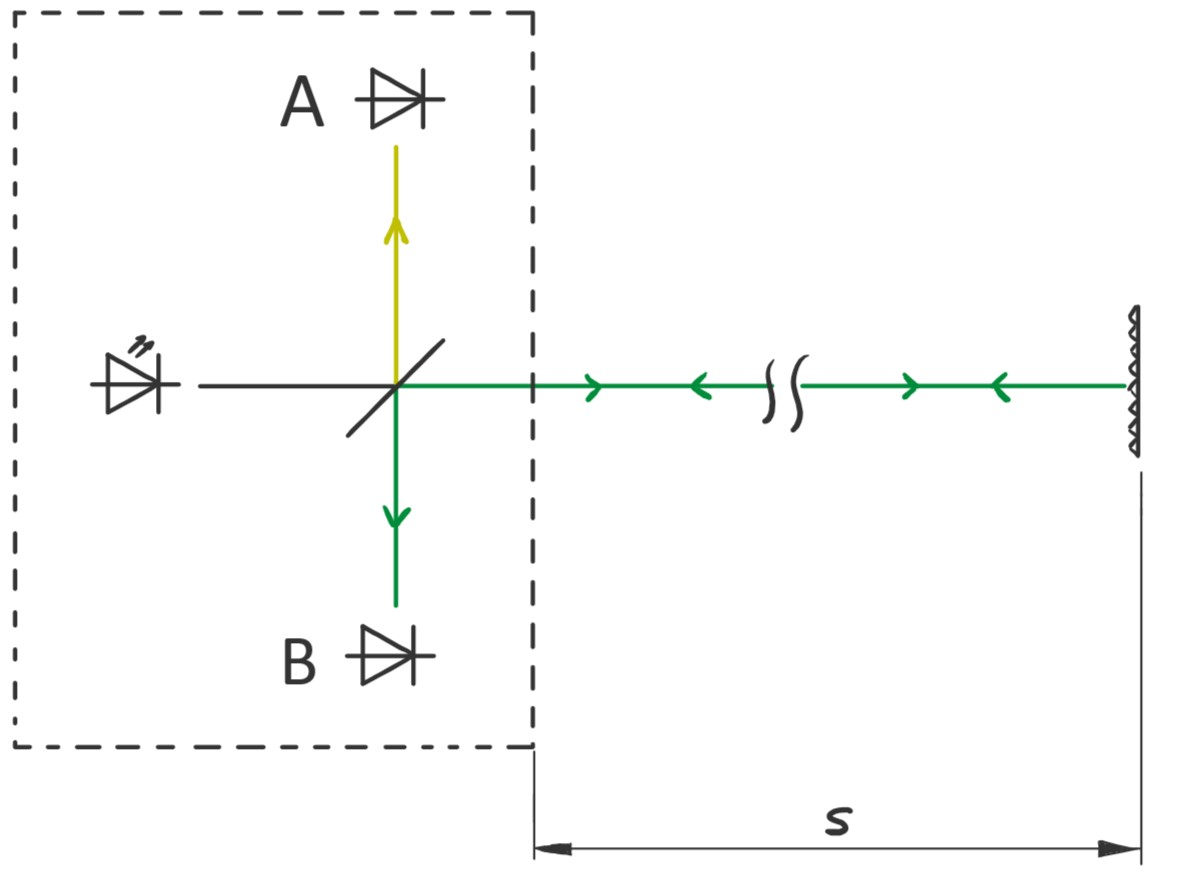
\includegraphics[width=.6\textwidth]{aufbau/strahlteilung.jpg}
    \caption[Skizze der Strahlgänge]{Skizze der Strahlgänge mit den Photodioden A und B. Gemessen wird die Strecke \(s\) vom Ausgang der Pulsquelle bis zum Prismen-Reflektor.}
    \label{fig:strahlteilung}
\end{figure}
%
\begin{figure}[h]
    \centering
    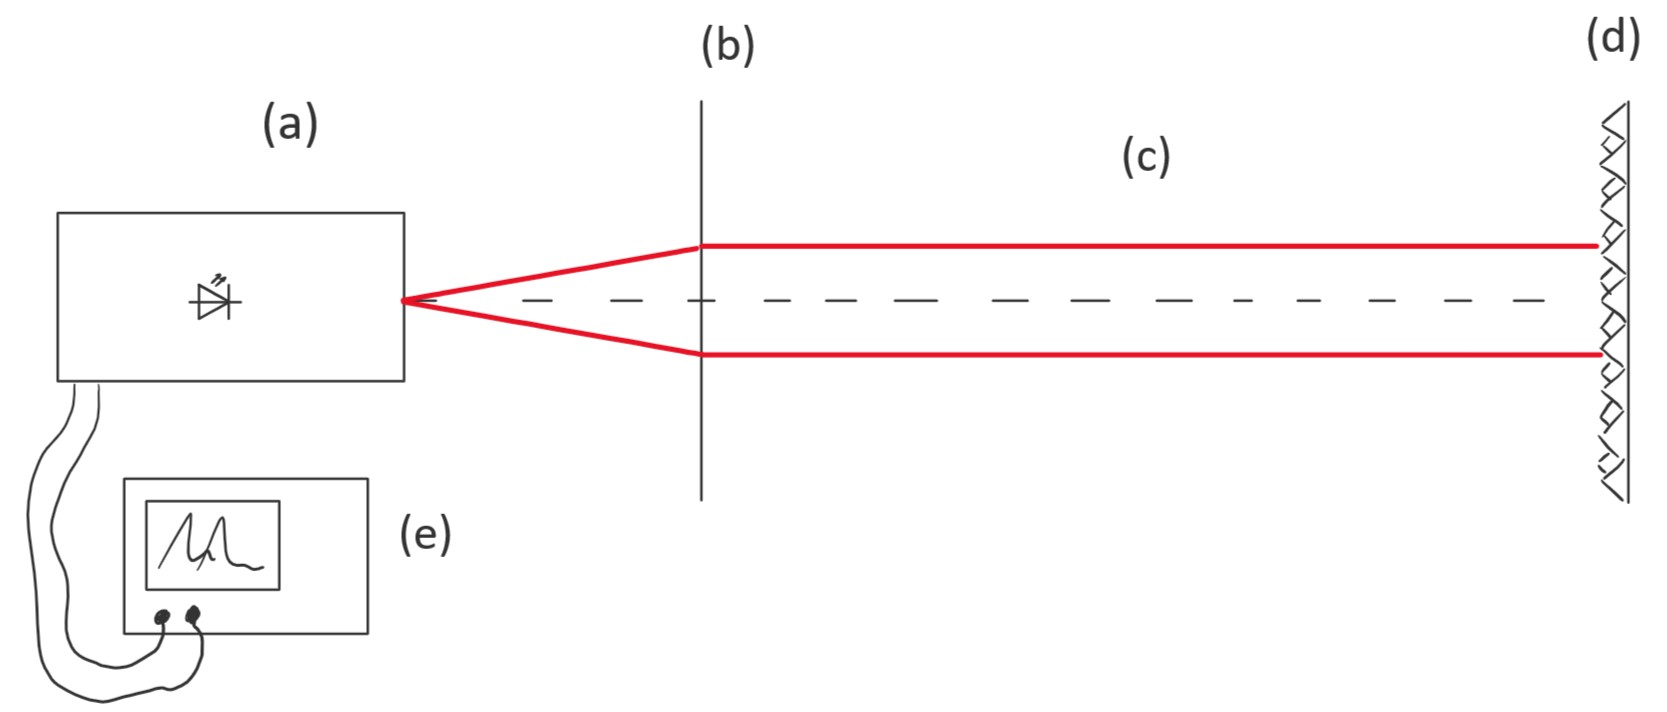
\includegraphics[width=.9\textwidth]{aufbau/devices.jpg}
    \caption[Anordnung der verwendeten Geräte]{Anordnung der verwendeten Geräte: (a) Pulsquelle mit Strahlteiler und Photodioden (b) \textsc{Fresnel}-Linse (c) Lichtstrahl (d) Prismen-Reflektor (e) Oszilloskop.}
    \label{fig:devices}
\end{figure}
%
Der in Photodiode A erzeugt Puls dient als Referenzimpuls. Da Licht keine instantane also endliche Wirkgeschwindigkeit
hat ist der in Photodiode B erwartete Puls durch die größere zurückgelegte Strecke gegenüber dem Referenzimpuls um die
Zeitdifferenz \(\Delta t\) phasenverschoben. Diese Differenz ist durch
\begin{equation}
    \Delta t = \frac{1}{c} \Delta s
\end{equation}
proportional zur Streckenänderung \(\Delta s\) mit \(c^{-1}\) als Proportionalitätsfaktor. Das erwartete Oszillogram ist
in \bild{fig:puls_skizze} dargestellt.\par
\begin{figure}[h]
    \centering
    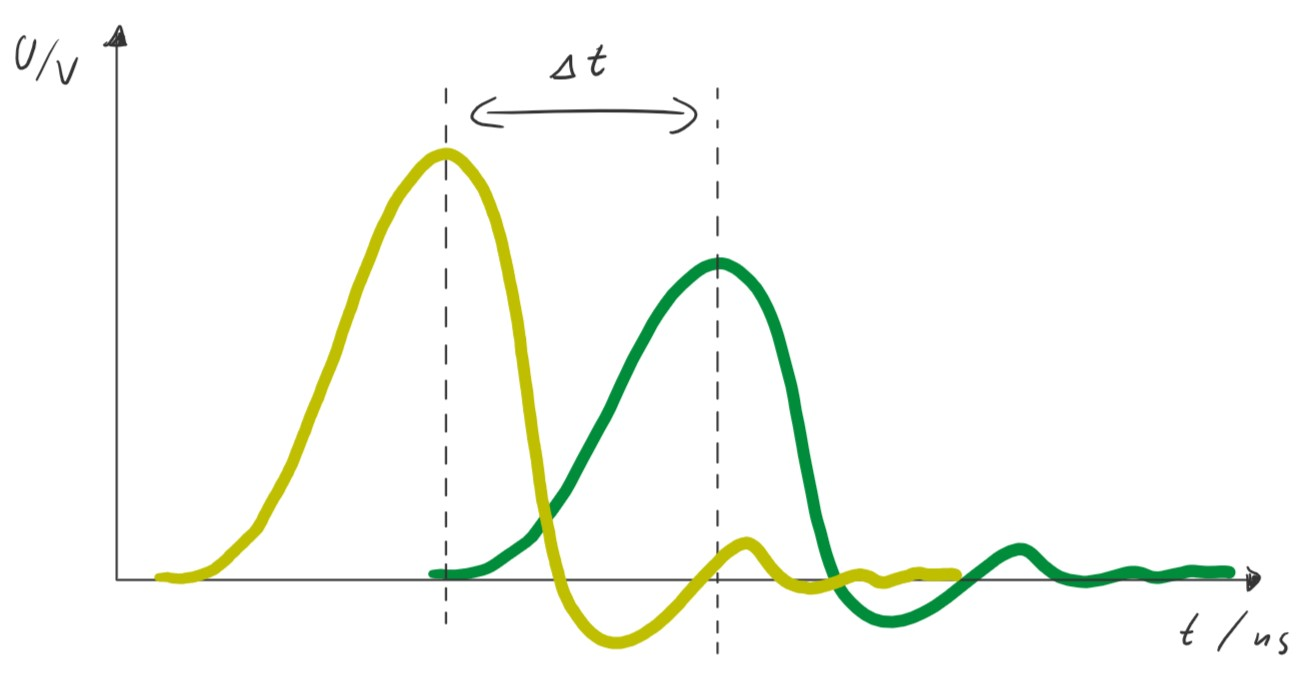
\includegraphics[width=.9\textwidth]{aufbau/signal_skizze_wht.jpg}
    \caption[Schematische Darstellung des erwarteten Oszillograms]{Schematische Darstellung des erwarteten Oszillograms.
            Referenzpuls in gelb und der um \(\Delta t\) phasenverschobene Puls des Messsignals in grün. Durch Streuung und
            Intensitätsverluste in den optischen Medien ist die Amplitude des Messignals um \(\Delta U\) geringer. Dies
            ist für den Versuch allerdings irrelevant.}
    \label{fig:puls_skizze}
\end{figure}
\input{chapters/4_durchführung}
\chapter{Auswertung}
Zur Bestimmung der Geschwindigkeit des Lichtes ist zu beachten, dass der Strahl die Strecke \(s\) auf dem Hin- und auf
dem Rückweg jeweils ein mal durchläuft. Die Streckenänderung \(\Delta s\) geht also mit einem Faktor 2 in die Berechnung
ein.
%
%=================================================================
%
\section{Lichtgeschwindigkeit}
Werden die im Versuch gemessenen Werte für die Laufzeitdifferenz \(\Delta t\) über den Strahlweg \(s\) des Messsignals aufgetragen,
so kann die Steigung der Ausgleichsgeraden als Kehrwert der Lichtgeschwindigkeit in \(\frac{m}{ns}\) interpretiert werden.
\begin{figure}[h]
    \centering
    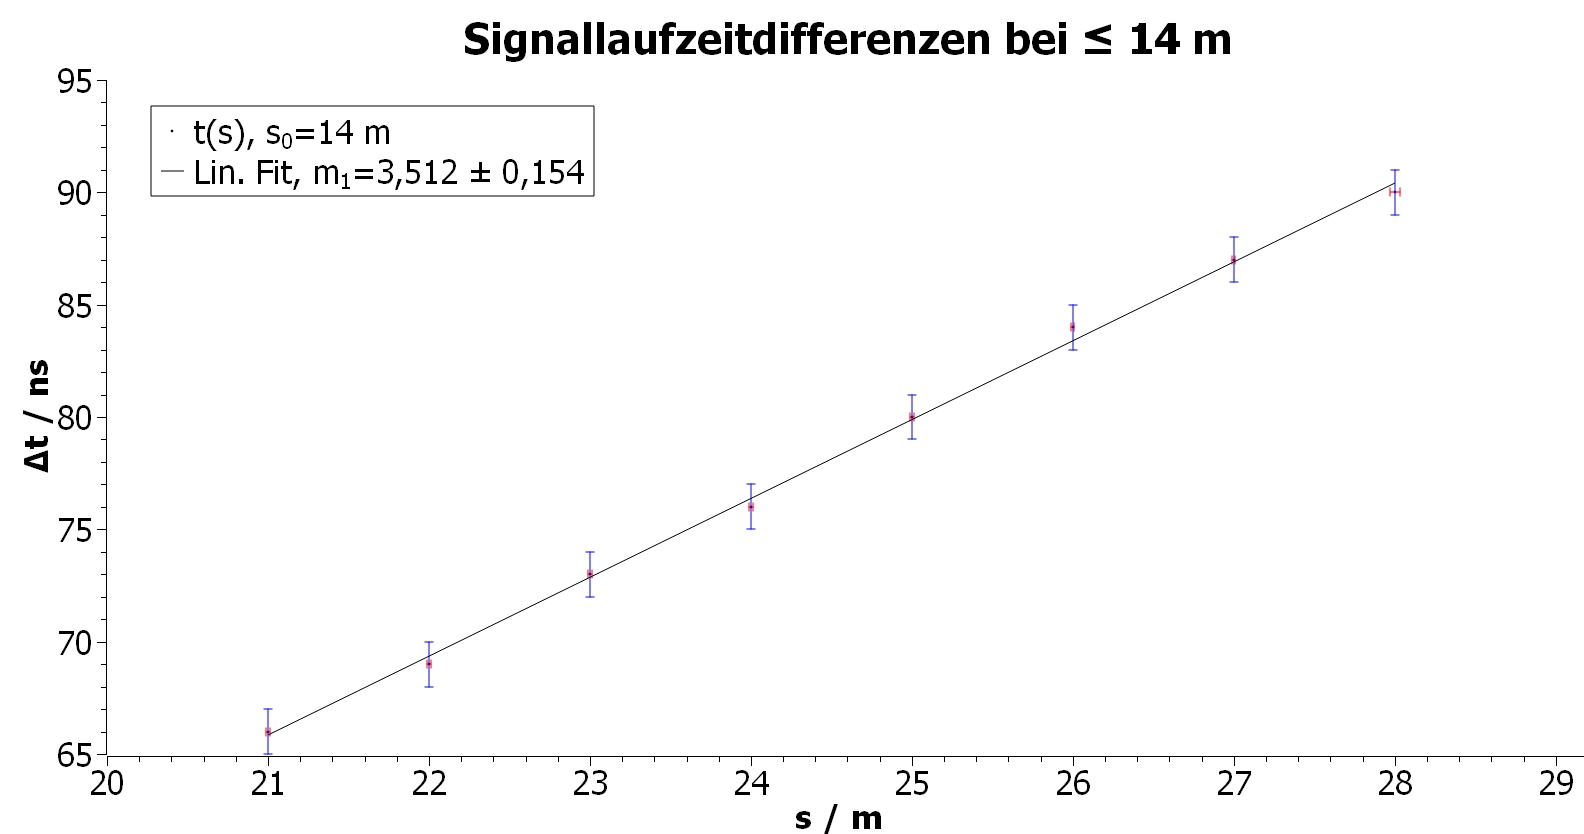
\includegraphics[width=.9\textwidth]{scidavis/14m.jpeg}
    \caption[Signallaufzeitunterschiede mit \(s_0 = \SI{14}{m}\)]{\(\Delta t(s)\)-Diagram im Intervall \( \SI{10,5}{m} \leq s \leq \SI{14}{m}\) mit \(s_0=\SI{14}{m}\).}
    \label{fig:14m}
\end{figure}
%
\begin{figure}[h]
    \centering
    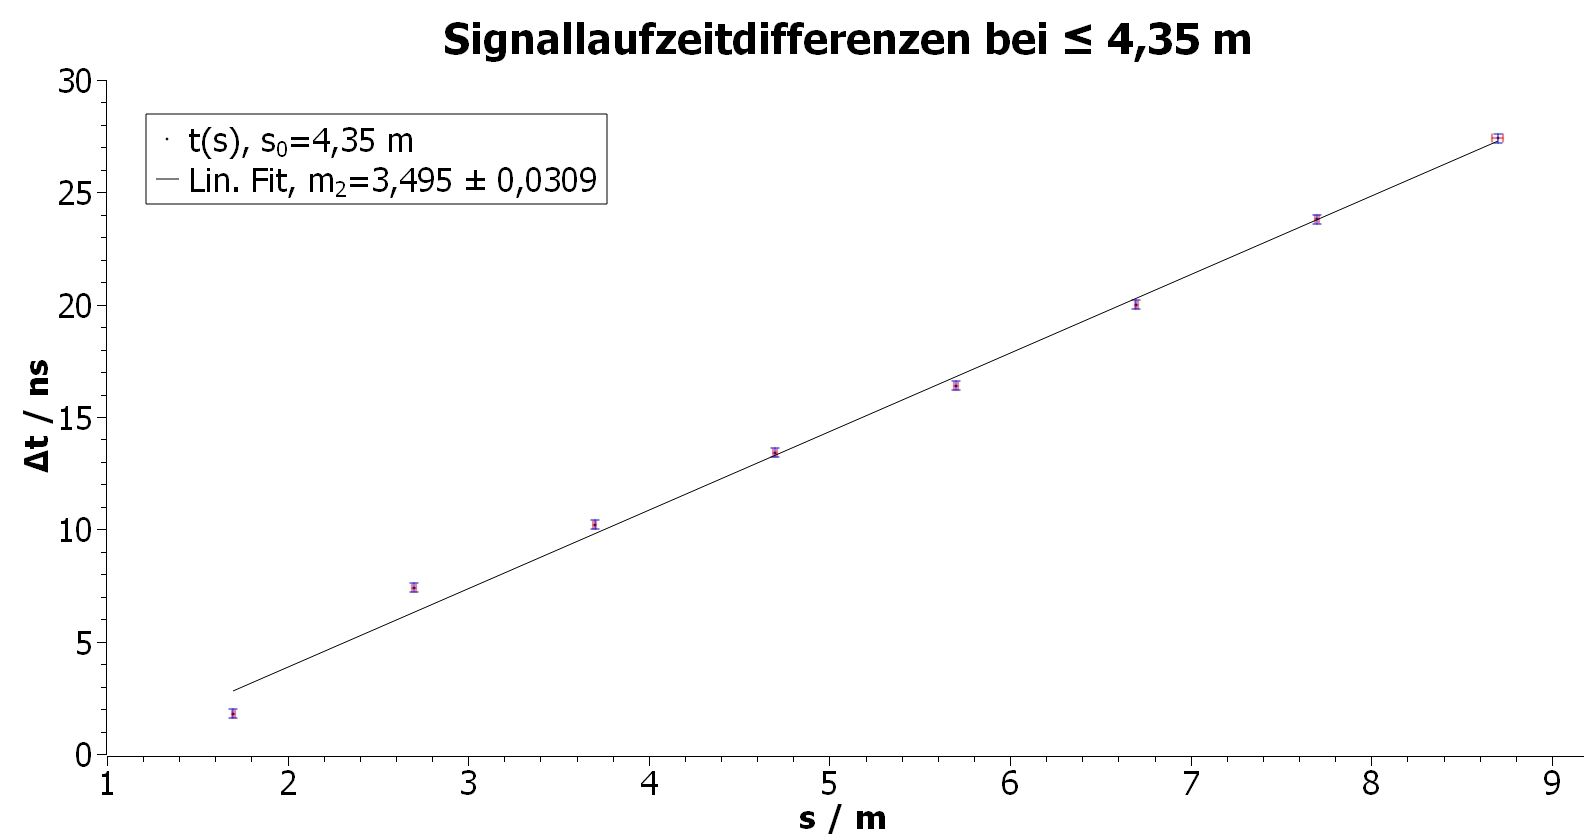
\includegraphics[width=.9\textwidth]{scidavis/4.35m.jpeg}
    \caption[Signallaufzeitunterschiede mit \(s_0 = \SI{4,35}{m}\)]{\(\Delta t(s)\)-Diagram im Intervall \( \SI{0,85}{m} \leq s \leq \SI{4,35}{m}\) mit \(s_0=\SI{4,35}{m}\).}
    \label{fig:4.35m}
\end{figure}
%
\bild{fig:14m} zeigt die Messung bei einer Anfangsdistanz des Prismen-Reflektors zur Strahlquelle von \SI{14}{m} unter einer Reduktion
der Distanz in Schritten von \SI{0,5}{m} bis herunter zu \SI{10,5}{m}. \bild{fig:4.35m} entsprechend die Messung bei einer
Anfangsdistanz von \SI{4,35}{m} herunter zu \SI{0,85}{m} bei gleicher Schrittweite. Prakmatische Limitierungen der
Versuchsumgebung - eine \glqq{}Lücke\grqq{} zwischen den Labortischen - ließen keine kontinuierliche Messungen im Bereich
zwischen \(\SI{10,5}{m} \text{ und } \SI{4,35}{m}\) zu.\par
Die Steigung der Ausgleichsgeraden \(m_{1,2}\) der Diagramme in \bild{fig:14m} und \bild{fig:4.35m} kann als Inverse der
Lichtgeschwindigkeit mit
\begin{equation}
    m = \frac{\Delta t}{\Delta s} = c^{-1} \quad \Leftrightarrow \quad c = m^{-1}
    \label{eq:lightspeed}
\end{equation}
verstanden werden.\par
Die beiden Messreihen führen so zu Werten für die Lichtgeschwindigkeit in Luft von
\begin{equation}
    m_1^{-1} = c_1 = \left( \SI{3,512}{\frac{ns}{m}} \right)^{-1} = \SI{2,847 \cdot 10^8}{\frac{m}{s}}
\end{equation}
und
\begin{equation}
    m_2^{-1} = c_2 = \left( \SI{3,495}{\frac{ns}{m}} \right)^{-1} = \SI{2,861 \cdot 10^8}{\frac{m}{s}}
\end{equation}
%
\section{Brennweite der \textsc{Fresnel}-Linse}
Die Brennweite kann durch die Gegenstands- und Bildweite bestimmt werden. Gemessen wurde für die Gegenstandsweite $ g=(485\pm 5)\SI{}{mm} $ und für die Bildweite $ b=(470\pm 5)\SI{}{mm} $.\\
Nach \gl{eq:brenn} kann die Brennweite $ f $ wie folgt berechnet werden:
\begin{align}
    f = \left( \frac{1}{b} + \frac{1}{g} \right)^{-1} = \left( \frac{1}{\SI{470}{mm}} + \frac{1}{\SI{485}{mm}} \right)^{-1} = \SI{238,7}{mm}
    \label{eq:brenn_val}
\end{align}
Der rechnerische Wert für die Brennwete weicht um \((136,3 \pm 2,5)\SI{}{mm}\) oder \((36,3 \pm 0,6)\%\) von der Angabe des Herstellers $ f_{H}=\SI{375}{mm} $ ab.
%
\section{Abweichung der Lichtgeschwindigkeit}
Die Abweichungen der Lichtgeschwindigkeiten sind durch die Fehlerfortpflanzung der Steigungen folgendermaßen zu bestimmen:
\begin{align}
    \Delta c_{1}    &= \left\vert \frac{\partial c_{1}}{\partial m_{1}} \right\vert \cdot \Delta m_{1} = m_{1}^{-2} \cdot \Delta m_{1} \nonumber \\
                    &= \left( 3,512 \cdot 10^{-9} \SI{}{\frac{s}{m}} \right)^{-2} \cdot 0,154\cdot 10^{-9} \SI{}{\frac{s}{m}} \nonumber \\
                    &= 0,125\cdot 10^{8} \SI{}{\frac{m}{s}}
\end{align}
\begin{align}
    \Delta c_{2}    &= \left\vert \frac{\partial c_{2}}{\partial m_{2}} \right\vert \cdot \Delta m_{2} = m_{2}^{-2} \cdot \Delta m_{2} \nonumber \\
                    &= \left(3,495\cdot 10^{-9}\SI{}{\frac{s}{m}}\right)^{-2} \cdot 0,0309 \cdot 10^{-9} \SI{}{\frac{s}{m}} \nonumber \\
                    &= 0,025\cdot 10^{8} \SI{}{\frac{m}{s}}
\end{align}
Für die Lichtgeschwindigkeiten ergibt sich also:
\begin{align}
    c_{1} &= (2,85 \pm 0,13)\cdot 10^{8}\SI{}{\frac{m}{s}}\\
    c_{2} &= (2,86 \pm 0,03)\cdot 10^{8}\SI{}{\frac{m}{s}}
\end{align}
%
\section{Abweichung der Brennweite}
Der Fehler der Brennweite ist abhängig von den Abweichungen der Gegenstands- und Bildweite:
\begin{align}
    \Delta f    &= \left\vert \frac{\partial f}{\partial b} \right\vert \cdot \Delta b + \left\vert \frac{\partial f}{\partial g} \right\vert \cdot \Delta g = \frac{1}{b^{2}} \cdot \left(\frac{1}{b}+\frac{1}{g} \right)^{-2} \cdot \Delta b + \frac{1}{g^{2}} \cdot \left(\frac{1}{b}+\frac{1}{g} \right)^{-2} \cdot \Delta g \nonumber \\
                &= \frac{1}{(\SI{470}{mm})^{2}} \cdot \left(\frac{1}{\SI{470}{mm}}+\frac{1}{\SI{485}{mm}} \right)^{-2} \cdot \SI{5}{mm} + \frac{1}{(\SI{485}{mm})^{2}} \cdot \left(\frac{1}{\SI{470}{mm}}+\frac{1}{\SI{485}{mm}} \right)^{-2} \cdot \SI{5}{mm} \nonumber \\
                &=\SI{1,29}{mm}+\SI{1,21}{mm} \nonumber \\
                &=\SI{2,50}{mm}
\end{align}
Die ermittelte Brennweite ist demnach:
\begin{equation}
    f=(238,7 \pm 2,5)\SI{}{mm}
\end{equation}
\chapter{Fazit}
Die Justage des optischen Systems um ein Signal sichtbar zu machen war zu Begin sehr umständlich. Nicht nur waren durch
den übrigen Laborbetrieb des öfteren Personen im Strahlweg, auch mussten wir um die sonstige Laboreinrichtung nicht zu
beschädigen mit einem erhöhten Maß an Geschicklichkeit aufwarten. Durch die beschriebene \glqq{}Lücke\grqq{} zwischen
den Labortischen musste der Aufbau zwei mal durchgeführt werden. Hier wäre ein Aufbau entlang einer Laborwand
möglicherweise geschickter. Einerseits würde es sekundäre Komplikationen minimieren und andererseits ermöglicht es eine
kontinuierliche, \glqq{}Lückenlose\grqq{} Reduktion der Strecke.\par
Sonst ist es aber ein schönes Experiment um ein \textit{leibhaftiges} Gefühl dafür zu bekommen, dass Licht sich in der
Tat mit endlicher Geschwindigkeit ausbreitet. Mit Blick auf die gemessenen Werte verblüfft es noch mehr, dass mit
vergleichsweise einfachen Mitteln die gemessene Lichtgeschwindigkeit in bodennaher Luft - durch den relativ geringen
Unterschied sicherlich auch auf eine Messung im Vakuum adaptierbar - mit einer Abweichung von \((5,1 \pm 4,3)\%\) für
\(c_1\) bzw. \((4,7 \pm 1)\%\) für \(c_2\) überraschend nah am rechnerischen Wert von \(\approx \SI{3 \cdot 10^{8}}{\frac{m}{s}}\)
(vgl. \gl{eq:brechung_luft}) liegen.\par\medskip
%
Die ermittelte Brennweite der Linse weicht von der Herstellerangabe deutlich ab, befindet sich allerdings noch im
plausiblen Bereich. Der Fehler der ermittelten Brennweite deckt den Herstellerwert auch nicht ab. Das liegt daran, dass
für den Fehler nur die Abstandsabweichungen der Gegenstands- und Bildweite berücksichtigt wurden, weshalb der Fehler
relativ klein erscheint. Weitere vernachlässigte Abweichungen könnten zum Beispiel sein, dass das Auffangen des
Laserpunkts über ein größeres Intervall der Abstände möglich war, in unserem Fall jedoch nur ein (Abstands-)Punkt zur
Messung gewählt wurde.\par
%-------------------
\newpage
\listoffigures 
\listoftables
\addchap{Verwendete Symbole}
\begin{table}[h]
    \begin{tabular}{@{}ll@{}}
        $s$ & Strahlweg\\
        $t$ & Laufzeitdifferenz\\
        $c$ & Lichtgeschwindigkeit\\
        $g$ & Gegenstandsweite (Abstand Linsenhauptebene zum Gegenstand/zur Quelle)\\
        $b$ & Bildweite (Abstand Linsenhauptebene zum Bild)\\
        $f$ & Brennweite\\
        $v$ & Ausbreitungsgeschwindigkeit\\
        $f'$ & \\
        $m$ & Steigung der Ausgleichsgeraden\\
        $t_p$ & \\
        $t_{rise}$ & \\
        $f_p$ & \\
        $\hat{U}$ & \\
        $\Delta t$ & \\        
    \end{tabular}
    \label{tab:glossar}
\end{table}
\appendix
\chapter{Anhang}
\begin{table}[h]
    \centering
    \caption[Tabelle der Messwerte]{Tabelle der Messwerte.}
    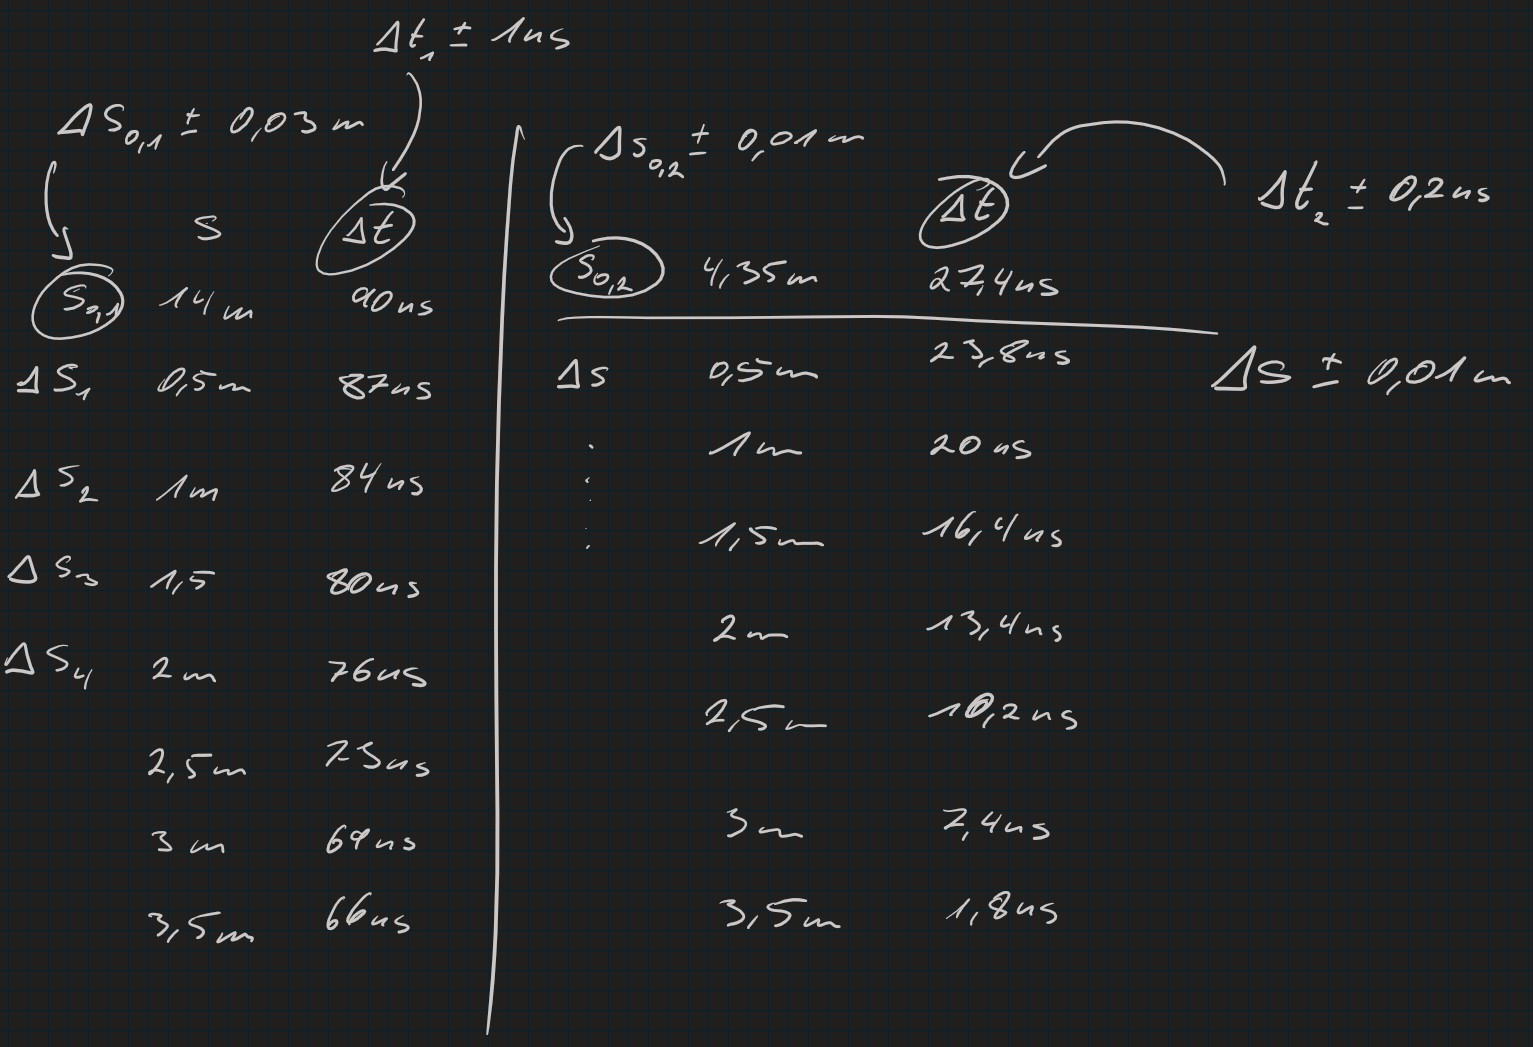
\includegraphics[width=\textwidth]{messungen/tabelle_messwerte.jpg}
    \label{tab:messwerte}
\end{table}
%
\begin{figure}[!ht]
    \centering
    \subfloat[\(\Delta t\)\label{subfig:delta_t}]{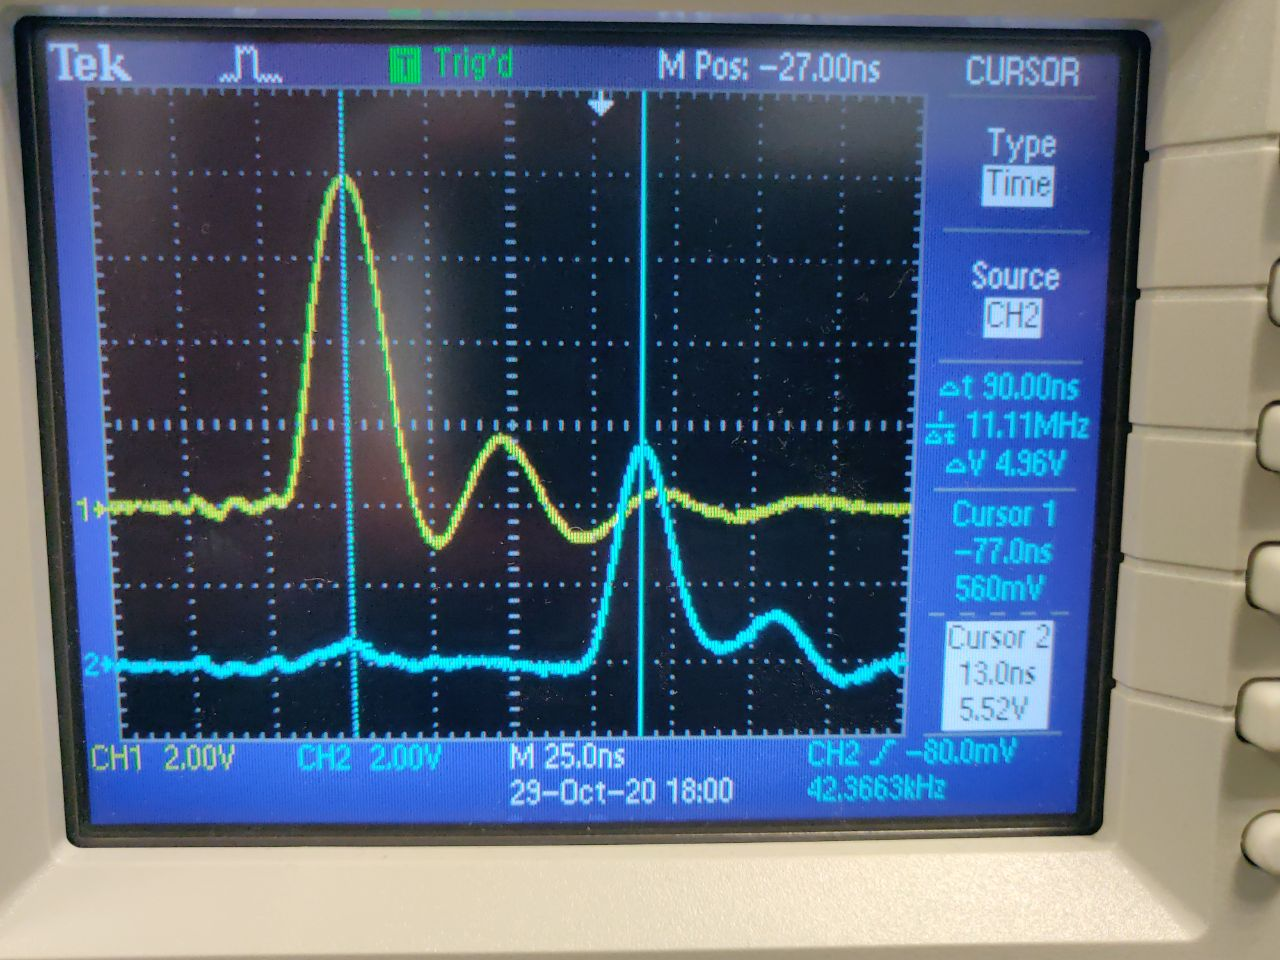
\includegraphics[width=0.45\textwidth]{messungen/delta_t.jpg}}
    \hspace{.05\textwidth}
    \subfloat[\(\hat{U}\)\label{subfig:U_dach}]{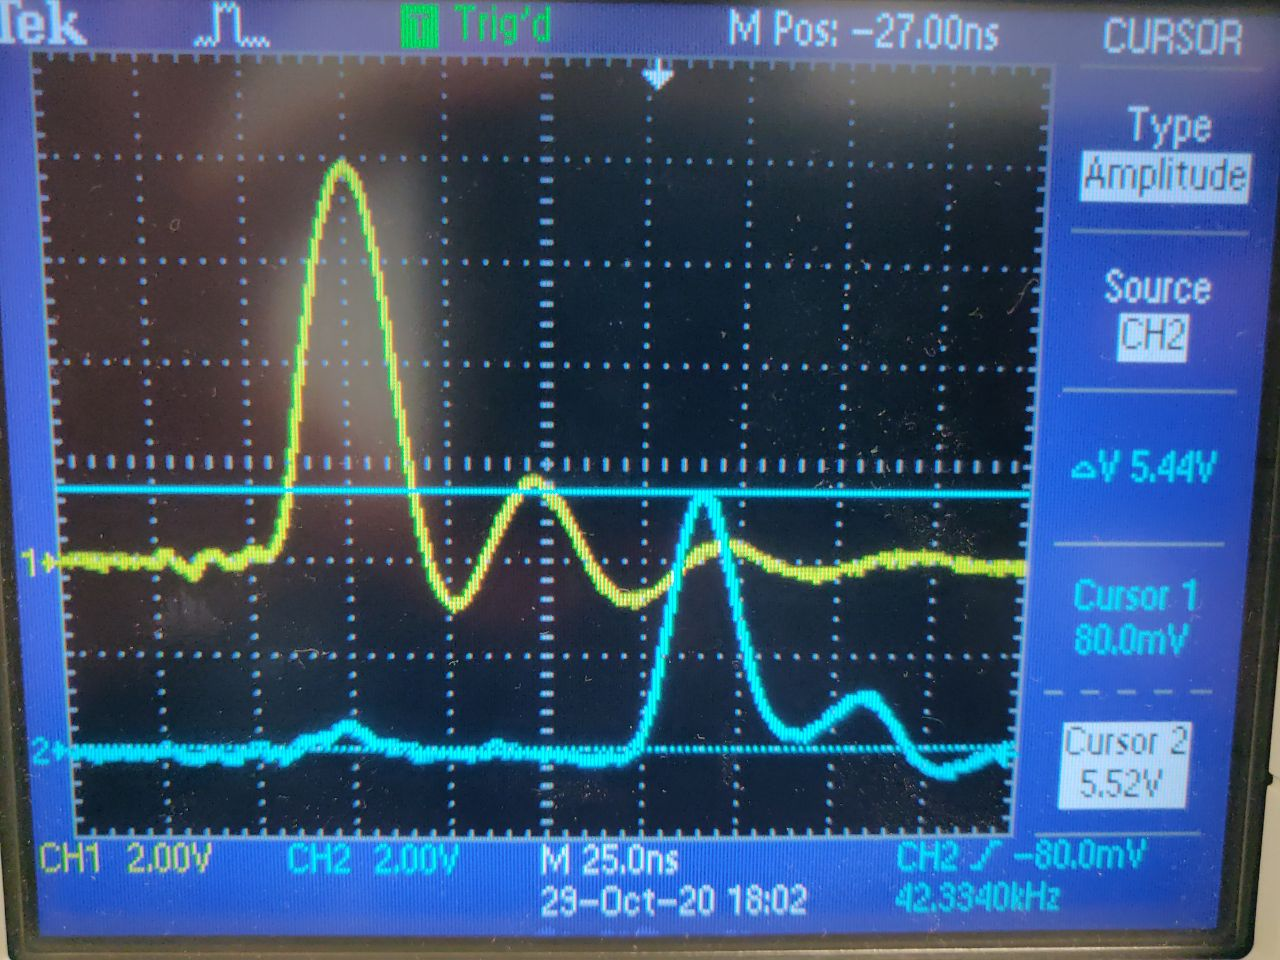
\includegraphics[width=0.45\textwidth]{messungen/U_dach.jpg}}
    \hspace{.2\textwidth}
    \subfloat[\(t_{rise}\)\label{subfig:t_rise}]{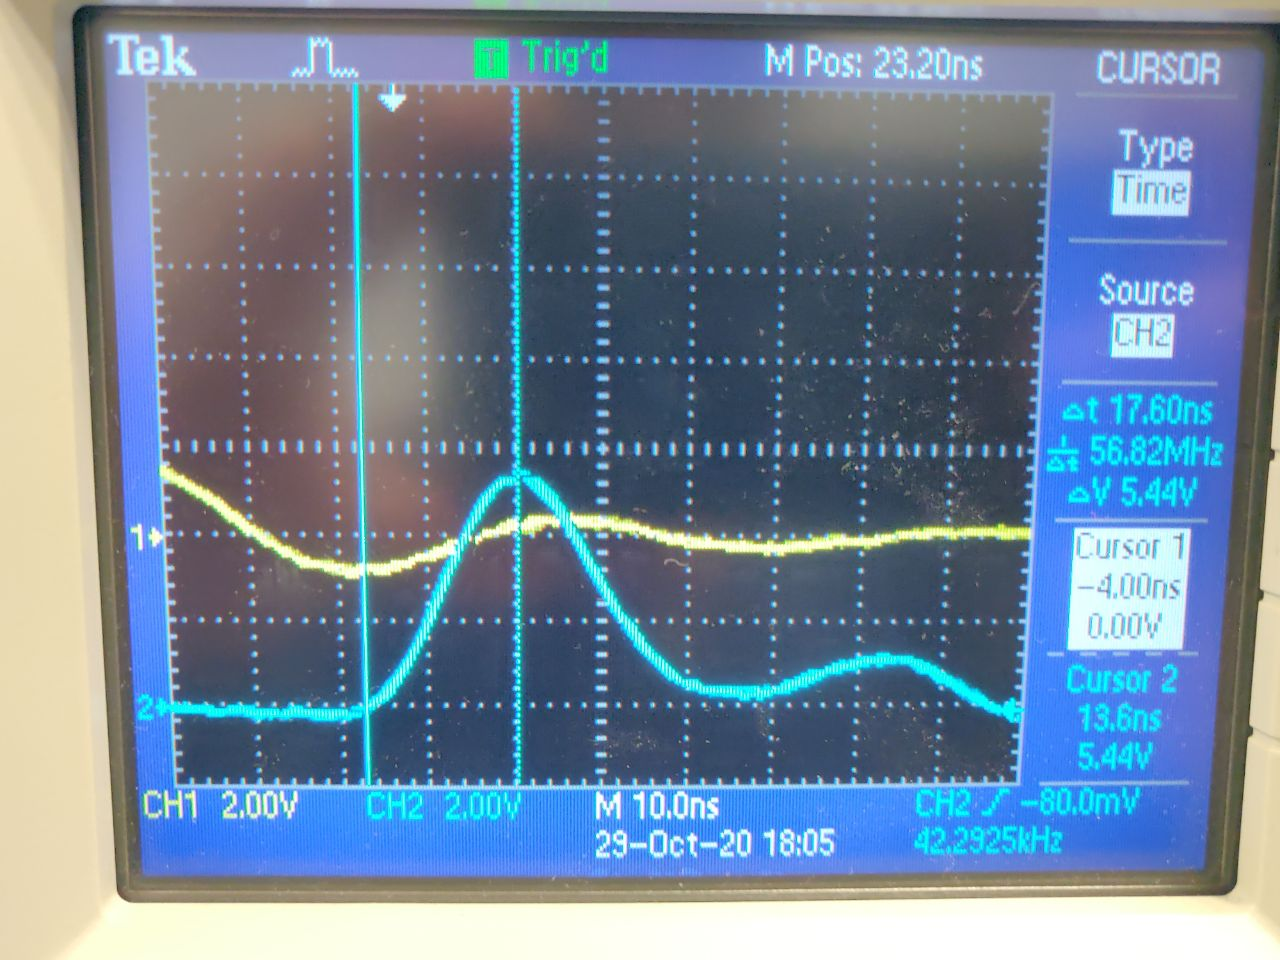
\includegraphics[width=0.45\textwidth]{messungen/t_rise.jpg}}
    \hspace{.05\textwidth}
    \subfloat[\(t_p\)\label{subfig:t_p}]{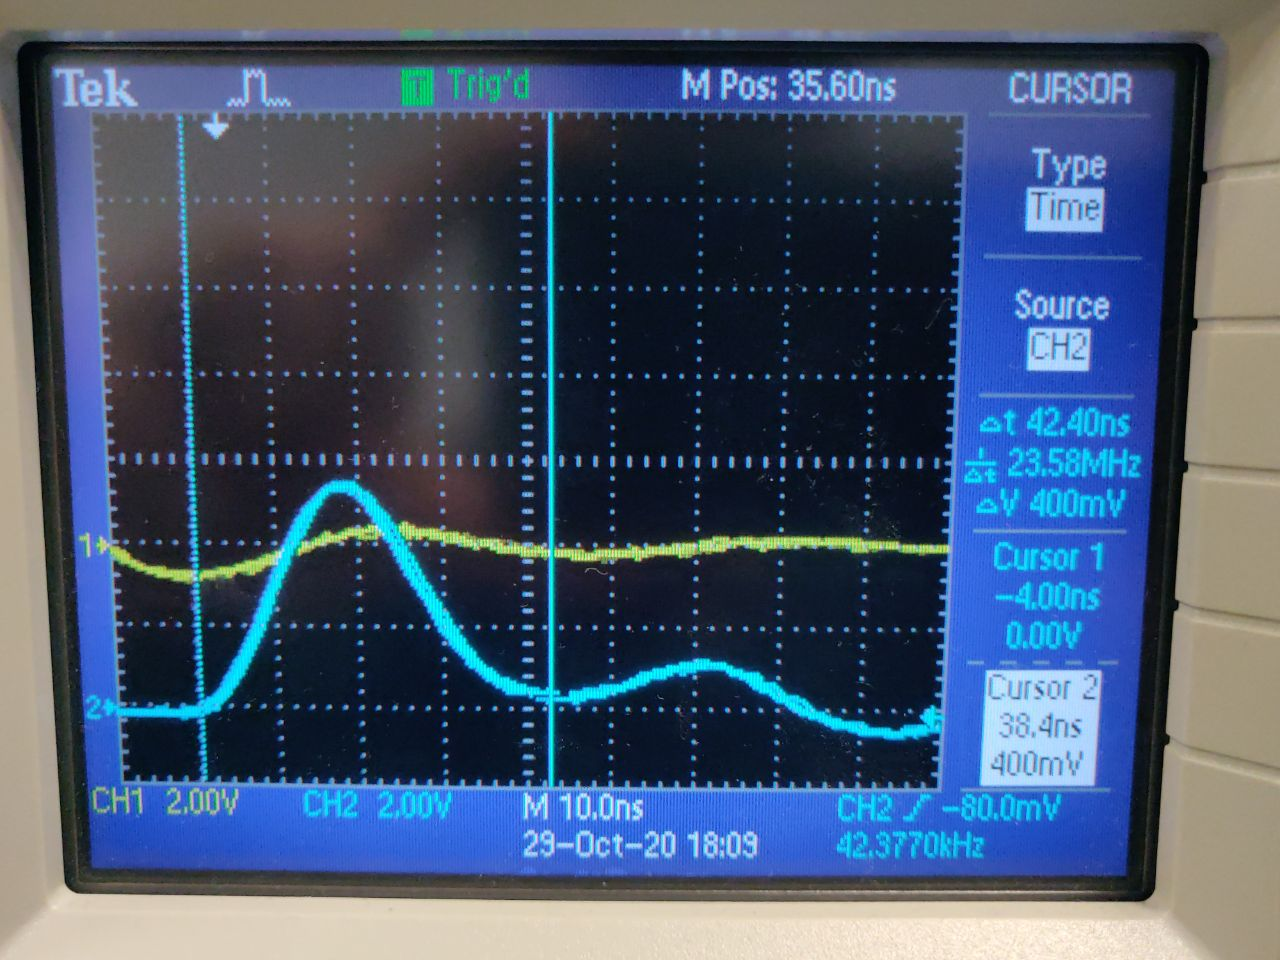
\includegraphics[width=0.45\textwidth]{messungen/t_pulse.jpg}}
    \hspace{.2\textwidth}
    \subfloat[\(f_p\)\label{subfig:f_p}]{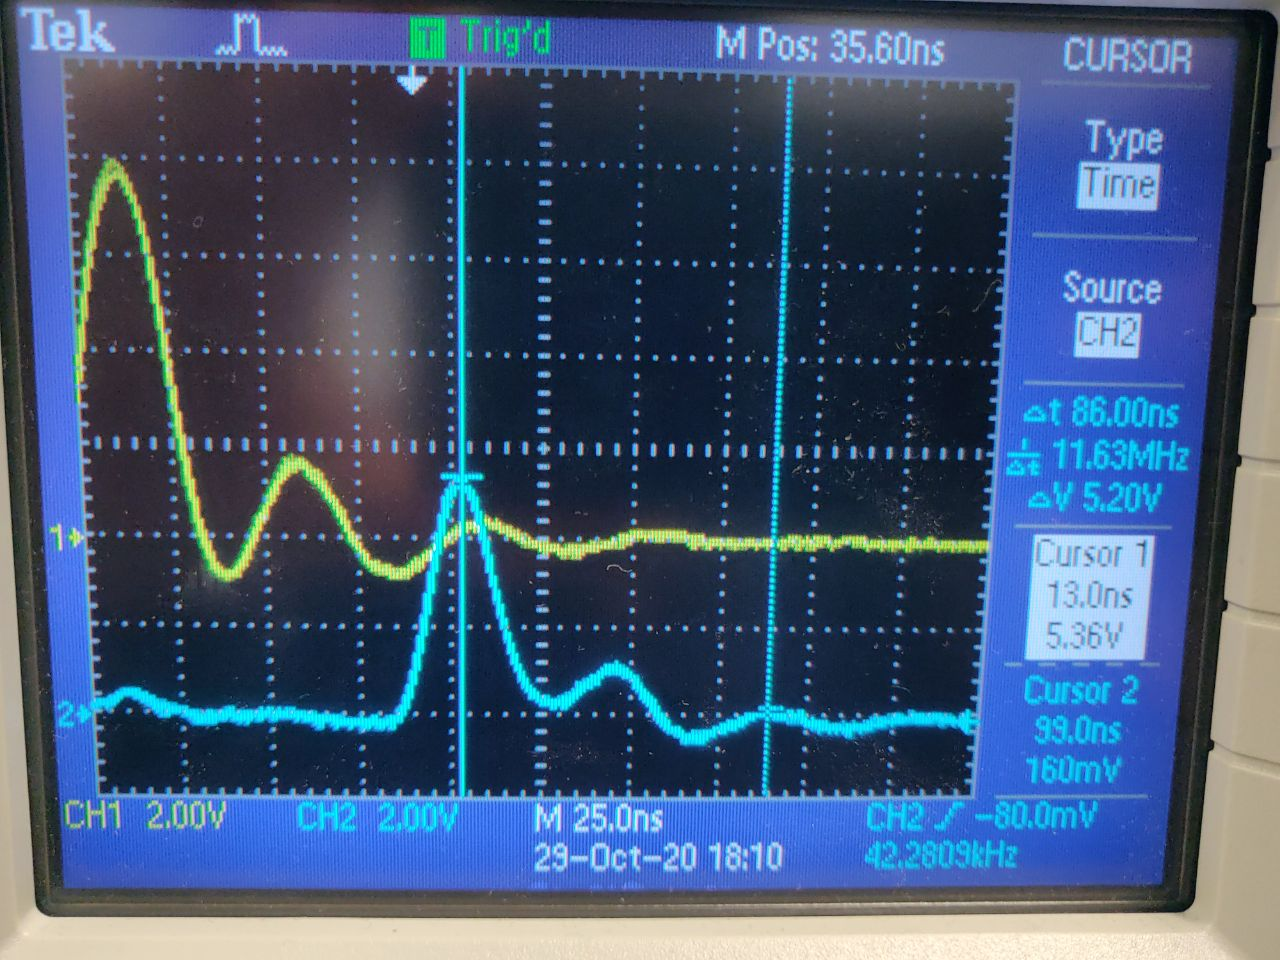
\includegraphics[width=0.45\textwidth]{messungen/freq_schwingung.jpg}}
    \caption[Oszillogramme]{Der Auswertung zu Grunde liegende Oszillogramme.}
 \end{figure}
\printbibliography
%\bibliographystyle{plaindin}
%==========================================
\end{document}